\begin{figure}
	\centering
	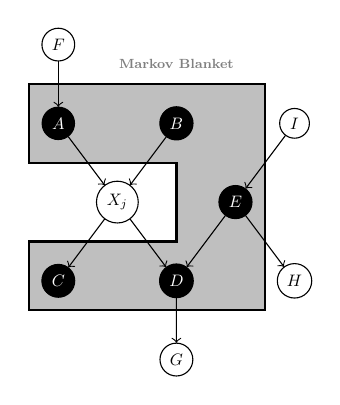
\begin{tikzpicture}[
		scale=0.5,
		every node/.style={scale=0.6}
	]
	
		\draw[thick,fill=lightgray] (-2.25,3) -- (3.75,3) -- (3.75,-2.75) -- (-2.25,-2.75)
			-- (-2.25,-1) -- (1.5,-1) -- (1.5,1) -- (-2.25,1) -- cycle;
	
		\node[circle,draw=black] (X) at (0,0) {$X_j$};
		
		\node[circle,draw=black,fill=black,text=white] (A) at (-1.5,2) {$A$};
		\node[circle,draw=black,fill=black,text=white] (B) at (1.5,2) {$B$};
		\node[circle,draw=black,fill=black,text=white] (C) at (-1.5,-2) {$C$};
		\node[circle,draw=black,fill=black,text=white] (D) at (1.5,-2) {$D$};
		\node[circle,draw=black,fill=black,text=white] (E) at (3,0) {$E$};

		\node[circle,draw=black] (F) at (-1.5,4) {$F$};
		\node[circle,draw=black] (G) at (1.5,-4) {$G$};
		\node[circle,draw=black] (H) at (4.5,-2) {$H$};
		\node[circle,draw=black] (I) at (4.5,2) {$I$};

		\draw[->] (A) -- (X);
		\draw[->] (B) -- (X);
		\draw[->] (X) -- (C);
		\draw[->] (X) -- (D);
		\draw[->] (E) -- (D);
		\draw[->] (F) -- (A);
		\draw[->] (D) -- (G);
		\draw[->] (E) -- (H);
		\draw[->] (I) -- (E);

		\node[gray] at (1.5,3.5) {\footnotesize \textbf{Markov Blanket}};
	\end{tikzpicture}
\end{figure}